Let 
\begin{align}
    \vec{A}=\myvec{1\\2}, \vec{B}=\myvec{3\\6}
\end{align}
Then from the equation of the line, 
\begin {align}
\vec{n^T} \vec {A}=c \label{july/1/76/eq:1} \\
\vec{n^T} \vec {B}=c  \label{july/1/76/eq:2} 
\end{align}
yielding
\begin{align}
    \vec{A}^T \vec {n}&=c \\
    \vec{B}^T \vec {n}&=c  \\
\implies     \myvec{\vec{A} \\ \vec{B}}^T \vec{n}&=c\myvec{1 \\ 1} \\
 \text{or, }  \myvec{1 &2 \\ 3&6} \vec{n}=\myvec{c\\c}
\end{align}
From the augmented matrix, 
\begin{align}
\myvec{ 1 &  2 & c \\ 3&  6& c } \xleftrightarrow{{3R_1-R_2\rightarrow R_2}} \myvec{ 1 &  2& c\\0 &  0 & -2c }
\end{align}
Thus,  the given system of lines has solution iff  $c = 0$  and the points are collinear.  This results in 
\begin{align}
    \myvec{ 1 &  2& 0\\0 &  0 & 0 } \\
\text{or, }    \myvec{1&2}\vec{n}=0
\implies \vec{n}= \myvec{-2\\1}
\end{align}
Thus, the desired equation of the straight line is 
\begin{align}
    \myvec{-2&1} \vec{x}=0 
\end{align}
\begin{figure}[H]
\centering
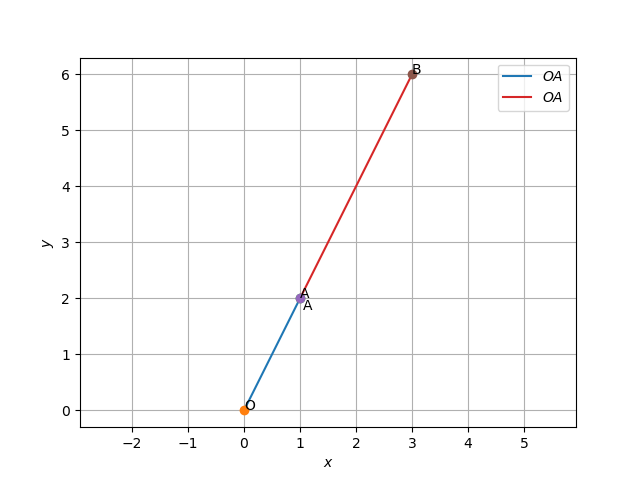
\includegraphics[width=\columnwidth]{github/ncert/linalg/matrices/solutions/july/det/76/1/Figure_1.png}
\caption{line formed with points \myvec{1&2} and \myvec{3&6} using Python}
\label{july/1/76/fig:1}
\end{figure}